\subsection{KNN Results}

%\mmt{We are only using 5 features, the independent variables: 
%\begin{equation*}
	%\big[m_1,m_2,\chi_1,\chi_2, \rm{SNR}\big]\,.
%\end{equation*}}

%\subsubsection{Finding the optimal hyperparameters}

We apply cross validation in order to fix the different hyperparameters of the algorithm.  To do so, we compute the score over a range of different parameters. We consider a number of neighbors between 1 and 20; the different metrics we test are the \texttt{euclidean}, \texttt{manhattan} and \texttt{cityblock}; the algorithms to compute the nearest neighbors can be \texttt{BallTree}, \texttt{KDTree} and the brute-force search, and the possible weight functions are the uniform weights (all points are weighted equally) and the \textit{distance} weights (points are weighted by the inverse of their distance). 

Considering all these possibilities, we apply the \texttt{cross val score} function from \texttt{scikit-learn} using a 10-fold cross validation to all the 23 datasets with different EOS.  We find that the optimal metric, algorithm and weights are the same for all the EOS, being the  \texttt{manhattan} metric, the \texttt{BallTree} algorithm (with a leaf size of 30) and the \textit{distance} weights. The only parameter that differs is the number of neighbors, that goes from 8 to 12. One can find the optimal hyperparameters and the corresponding score for each EOS in Table~\ref{tab:KNN_CV}. Doing an average weighting by the Bayes factor of each EOS, we finally get an optimal number of neighbors of 10. The mean score from the cross validation goes from 0.941 (for H4 EOS) to 0.953 (for APR4 EPP), as one can see in Table~\ref{tab:KNN_CV}.  

\begin{table}
    \centering
\begin{tabular}{cccc}
\hline
    EOS & Score & $K_{\rm neighbors}$ & Bayes Factor\\
    \hline 
    \hline
    APR4 EPP & 0.953 & 10 &  1.526 \\
    BHF BBB2 & 0.951 & 8  &  1.555 \\
    H4       & 0.941 & 10 &  0.056 \\
    HQC18    & 0.950 & 10 &  1.422 \\
    KDE0V    & 0.951 & 8  &  1.177 \\
    KDE0V1   & 0.949 & 10 &  1.283 \\
    MPA1     & 0.951 & 14 &  0.276 \\
    MS1 PP   & 0.948 & 12 &  0.001 \\
    MS1B PP  & 0.947 & 11 &  0.009 \\
    RS       & 0.945 & 10 &  0.176 \\
    SK255    & 0.946 & 10 &  0.179 \\
    SK272    & 0.945 & 10 &  0.156 \\
    SKI2     & 0.943 & 12 &  0.108 \\ 
    SKI3     & 0.943 & 12 &  0.107 \\
    SKI4     & 0.949 & 10 &  0.330 \\
    SKI5     & 0.945 & 9  &  0.025 \\
    SKI6     & 0.949 & 10 &  0.288 \\
    SKMP     & 0.948 & 10 &  0.290 \\
    SKOP     & 0.948 & 10 &  0.618 \\
    SLy      & 0.950 & 10 &  1.000 \\
    SLY2     & 0.950 & 10 &  1.028 \\
    SLY9     & 0.949 & 10 &  0.370 \\
    SLY230A  & 0.950 & 10 &  0.932 \\
    
\hline
\end{tabular}
    \caption{}
    \label{tab:KNN_CV}
\end{table}


Considering now the SLy EOS,  the model with these parameters gives a confusion matrix that is shown in Fig.~\ref{fig:KNN_confmat_SLY}.  The probability of having a NS as a function of $m_1$ and $m_2$  is shown in Fig.~\ref{fig:KNN_paramsweep_NS_SLY}. There are no big differences with different values of the spins, but the most remarkable one is that the model classifies better for 0-spin values, especially when $m_1$ is large.  There is also a dependence of the probability of having a remnant on the value of the spin that can be seen in Fig.~\ref{fig:KNN_paramsweep_REM_SLY}.This dependence is correct, since the probability of having a remnant increases for large values of $m_1$ at larger spin, but this dependence is given by the EOS. 

\begin{figure}
\centering
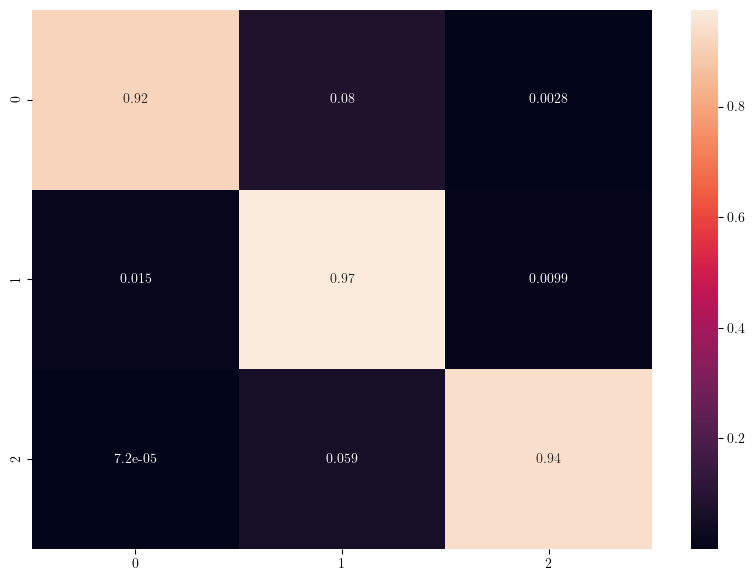
\includegraphics[width=0.45\textwidth]{/figs/KNN_confmat_SLy.png}
\caption{\label{fig:KNN_confmat_SLY} Confusion matrix SLy KNN}
\end{figure}

\begin{figure}
\centering
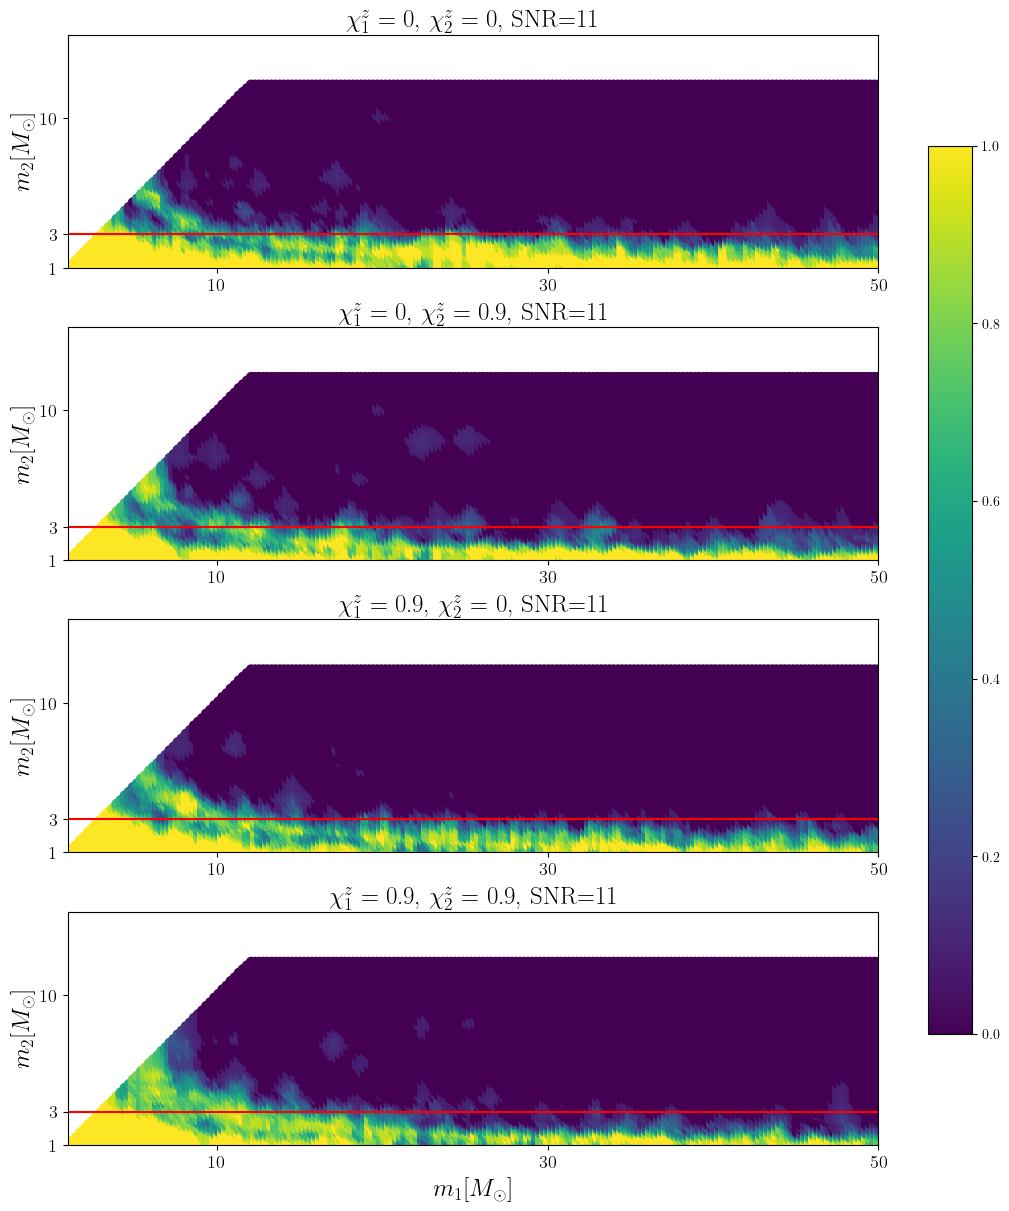
\includegraphics[width=0.45\textwidth]{/figs/KNN_param_sweep_spin_NS_SLy.png}
\caption{\label{fig:KNN_paramsweep_NS_SLY} Parameter sweep NS SLy KNN}
\end{figure}

\begin{figure}
\centering
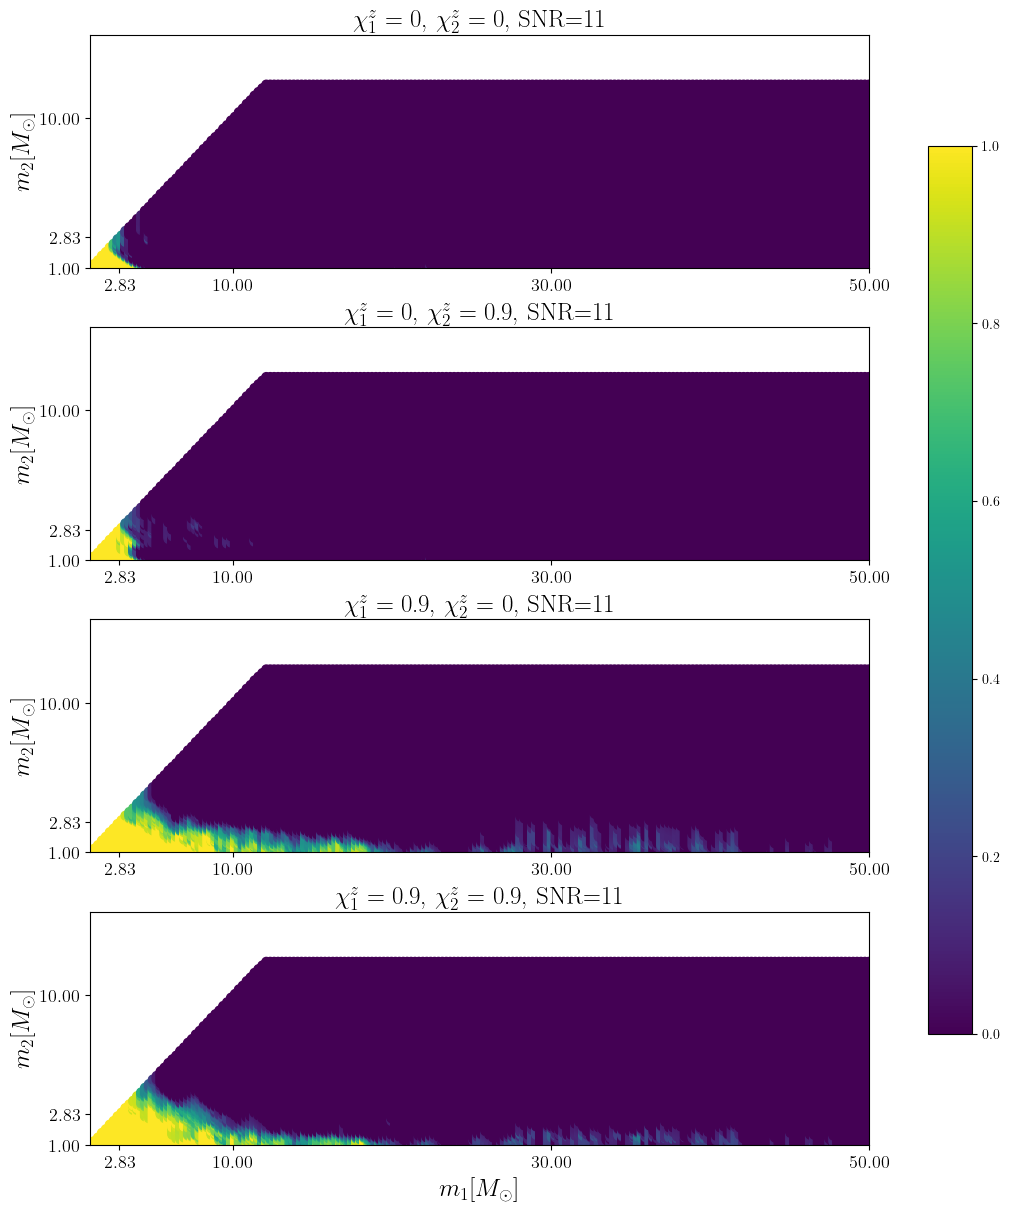
\includegraphics[width=0.45\textwidth]{/figs/KNN_param_sweep_spin_REM_SLy.png}
\caption{\label{fig:KNN_paramsweep_REM_SLY} Parameter sweep REM SLy KNN}
\end{figure}

In Figs.~\ref{fig:KNN_hist_BHFBBB2}, \ref{fig:KNN_hist_SLY} and \ref{fig:KNN_hist_MS1PP}  we depict the histograms of the probabilities p(\textit{HasNS}) (p(\textit{HasRemnant})) for injections of binaries that had a NS (EM counterpart) and for those that not, for the EOS BHF BB2, MS1 PP and SLy, respectively.

\begin{figure}
\centering
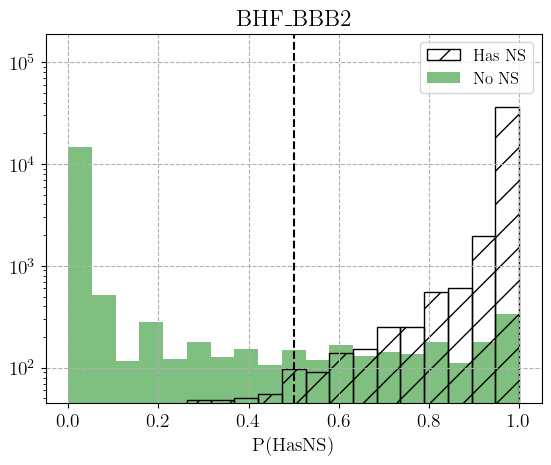
\includegraphics[width=0.45\textwidth]{/figs/KNN_BHF_BBB2_NShist.png}
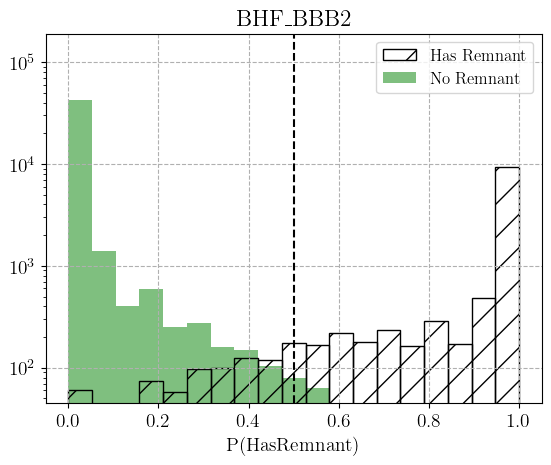
\includegraphics[width=0.45\textwidth]{/figs/KNN_BHF_BBB2_REMhist.png}
\caption{\label{fig:KNN_hist_BHFBBB2} Histograms BHF BBB2 KNN}
\end{figure}

\begin{figure}
\centering
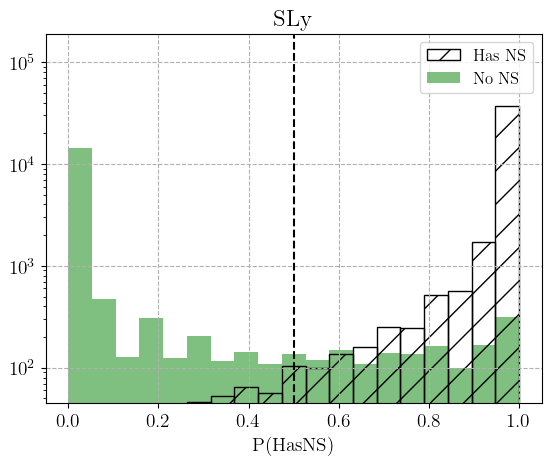
\includegraphics[width=0.45\textwidth]{/figs/KNN_SLy_NShist.png}
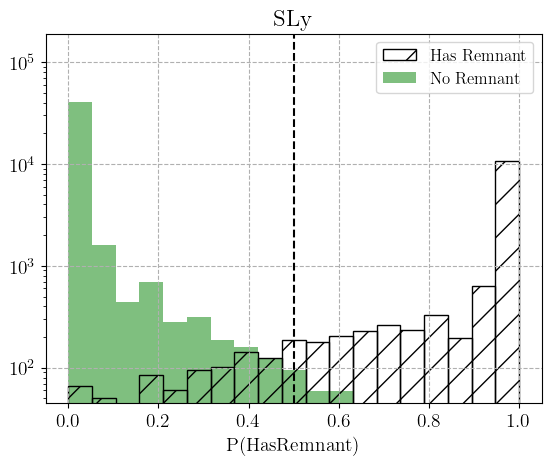
\includegraphics[width=0.45\textwidth]{/figs/KNN_SLy_REMhist.png}
\caption{\label{fig:KNN_hist_SLY} Histograms SLy KNN}
\end{figure}

\begin{figure}
\centering
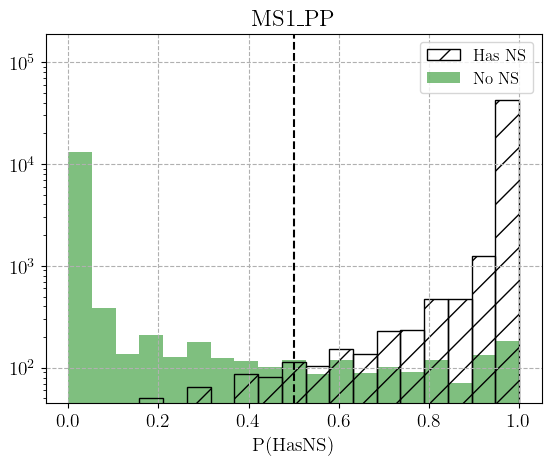
\includegraphics[width=0.45\textwidth]{/figs/KNN_MS1_PP_NShist.png}
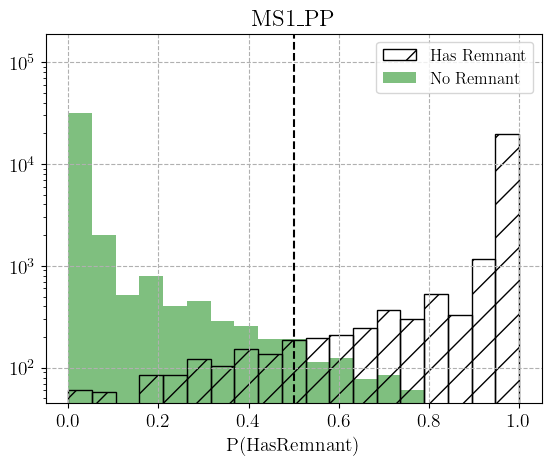
\includegraphics[width=0.45\textwidth]{/figs/KNN_MS1_PP_REMhist.png}
\caption{\label{fig:KNN_hist_MS1PP} Histograms MS1 PP KNN}
\end{figure}

We show in Fig.~\ref{fig:KNN_roc} the ROC curves of the classifier for the two different probabilities we consider. All the EOS are depicted in this figure, but we highlight three cases: BHF BBB2, MS1 PP and SLy.

\begin{figure}
\centering
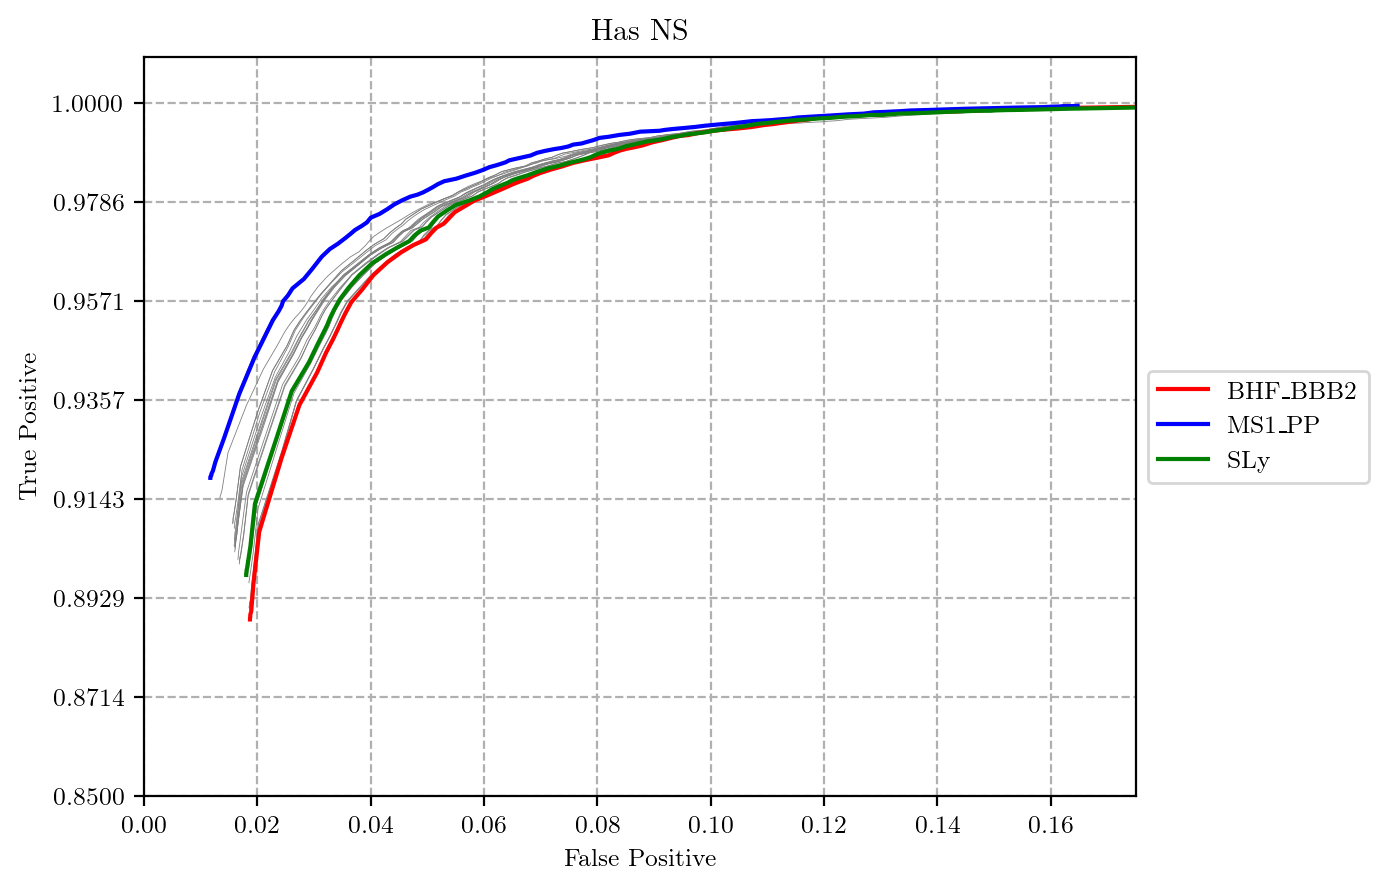
\includegraphics[width=0.45\textwidth]{/figs/ROC_KNN_NS.png}
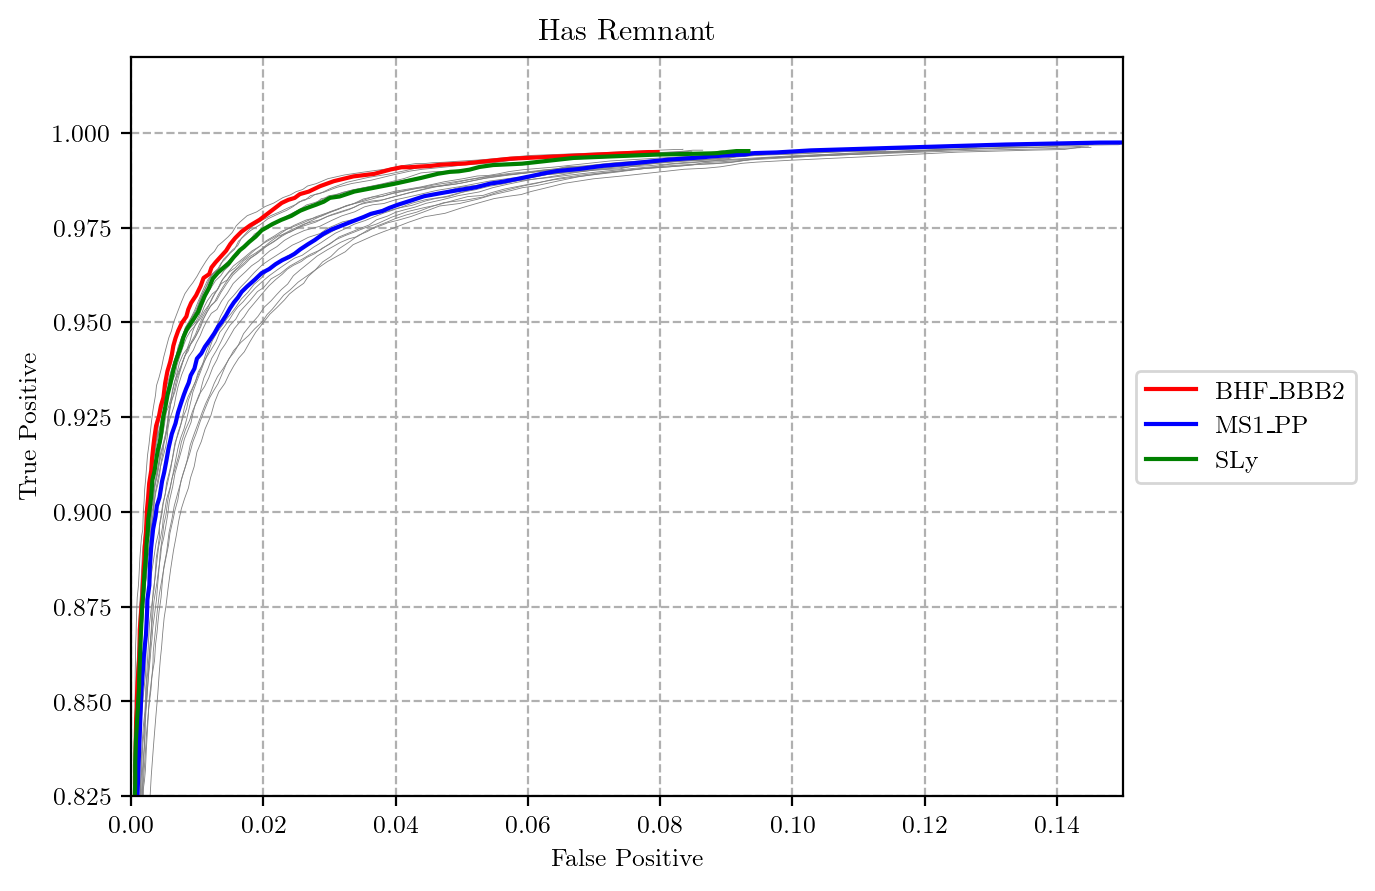
\includegraphics[width=0.45\textwidth]{/figs/ROC_KNN_REM.png}
\caption{\label{fig:KNN_roc} ROC curves KNN}
\end{figure}




%\subsubsection{\mmt{Has NS old}}
%\mmt{The metric we use to compute the distance between neighbors is the \textit{Manhattan} metric (or the Minkowski's $L1$ distance),  which is the distance between two points measured along axes at right angles. Having $p_1(x_1,y_1)$ and $p_2(x_2,y_2)$ the distance will be}
%\begin{equation}
%	d = |x_1-x_2|+|y_1-y_2|\,.
%\end{equation}

%\mmt{Moreover, the points are weighted uniformly.  After applying cross-validation,  we get that the optimal number of neighbors is $K_{\rm NS} = 10$, with a mean score $\rm{s_m} = 0:9718355224352762$ and a testing score  $\rm{s_t} = 0.9723828730478842$. In Fig.~\ref{fig:crossvalK} you can find how the mean score changes with the number of neighbors of the algorithm. } 

%\begin{figure}
  %  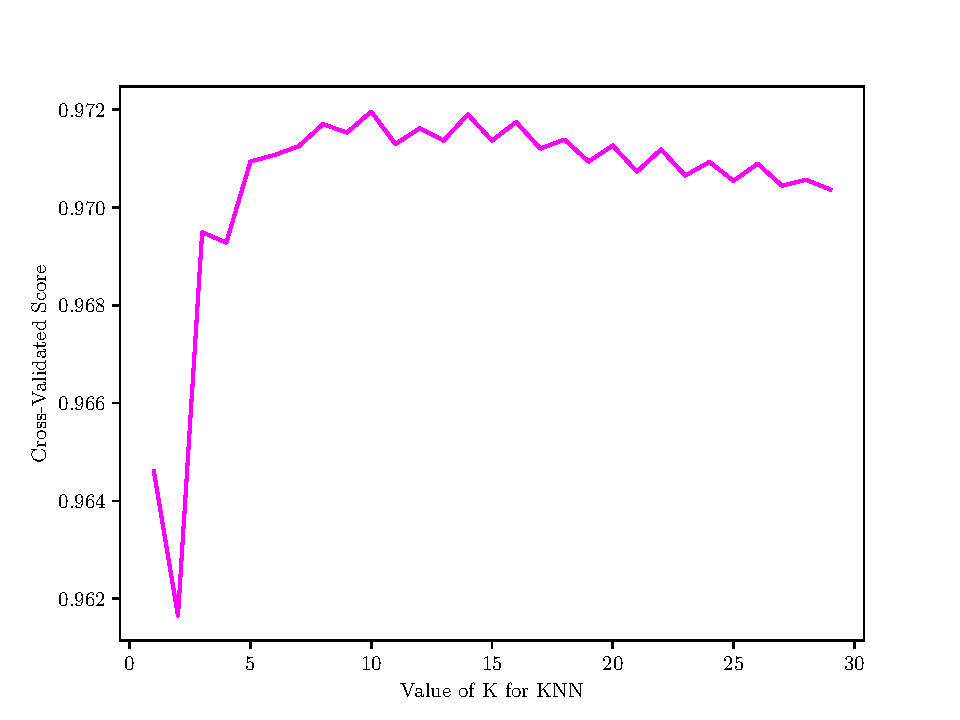
\includegraphics[width = 0.4\textwidth]{CrossValK.pdf}
  %  \caption{Score of our KNN model as a function of the number of neighbors. We are considering \textit{HasNS}.}
  %  \label{fig:crossvalK}
%\end{figure}
    
%\begin{figure}
  %  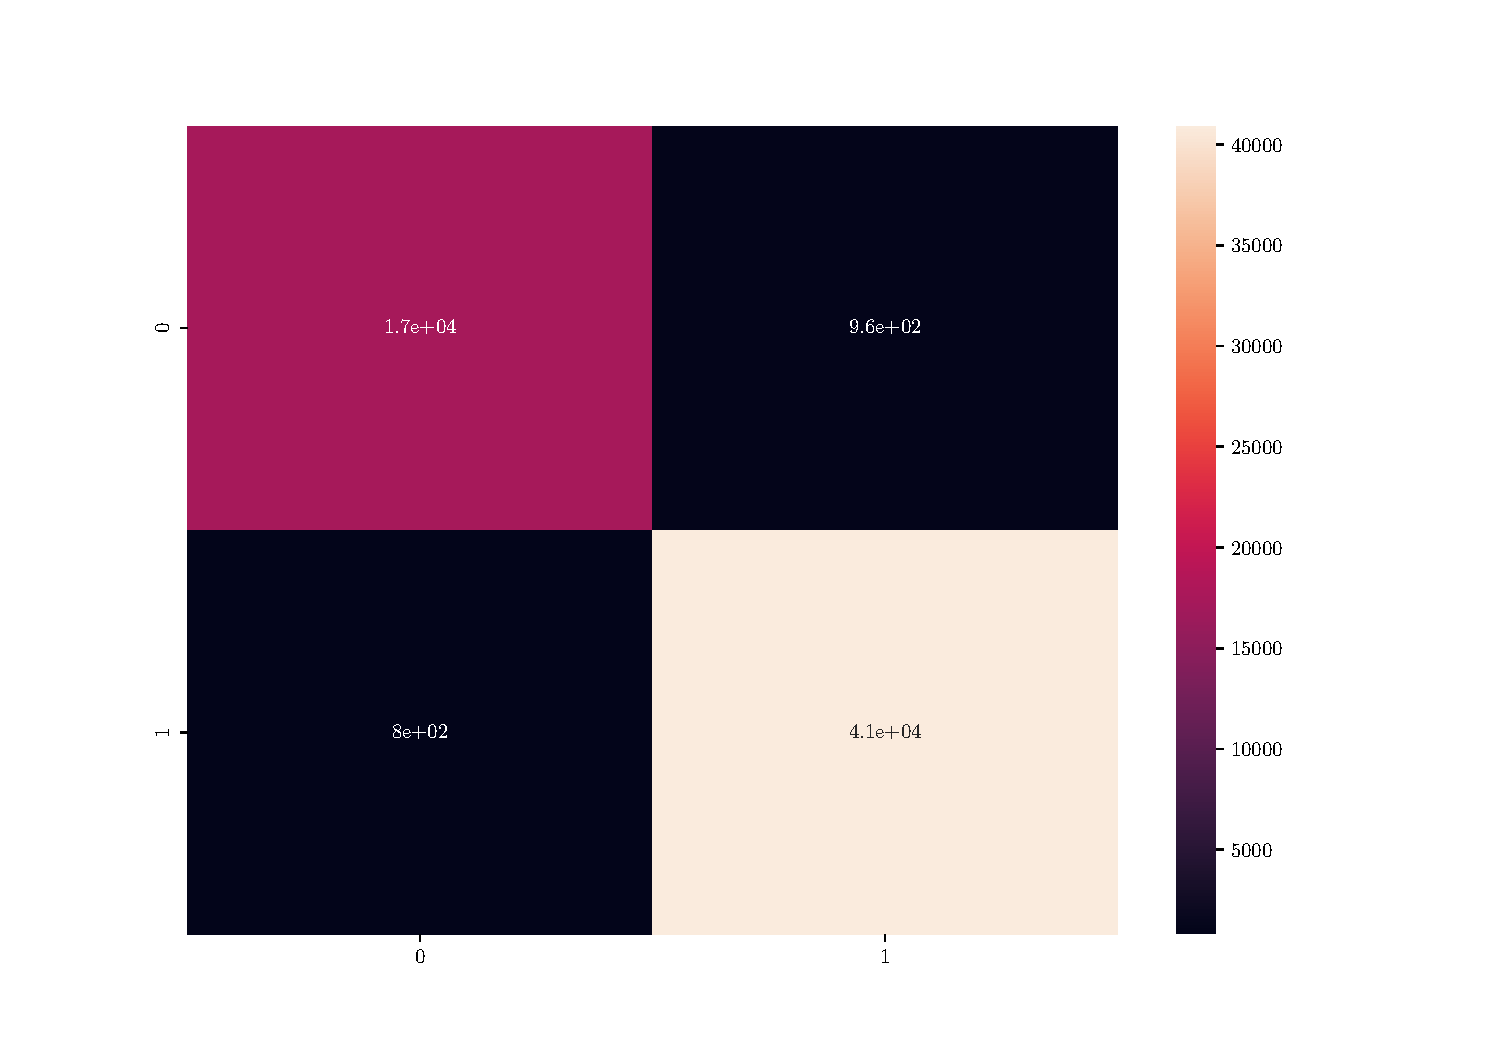
\includegraphics[width=0.45\textwidth]{conf_matrix_NS.pdf}
  %  \caption{Confusion matrix for our model for \textit{HasNS}, using the independent %recovered values. }
  %  \label{fig:confmat}
%\end{figure}

%\begin{figure}
  %  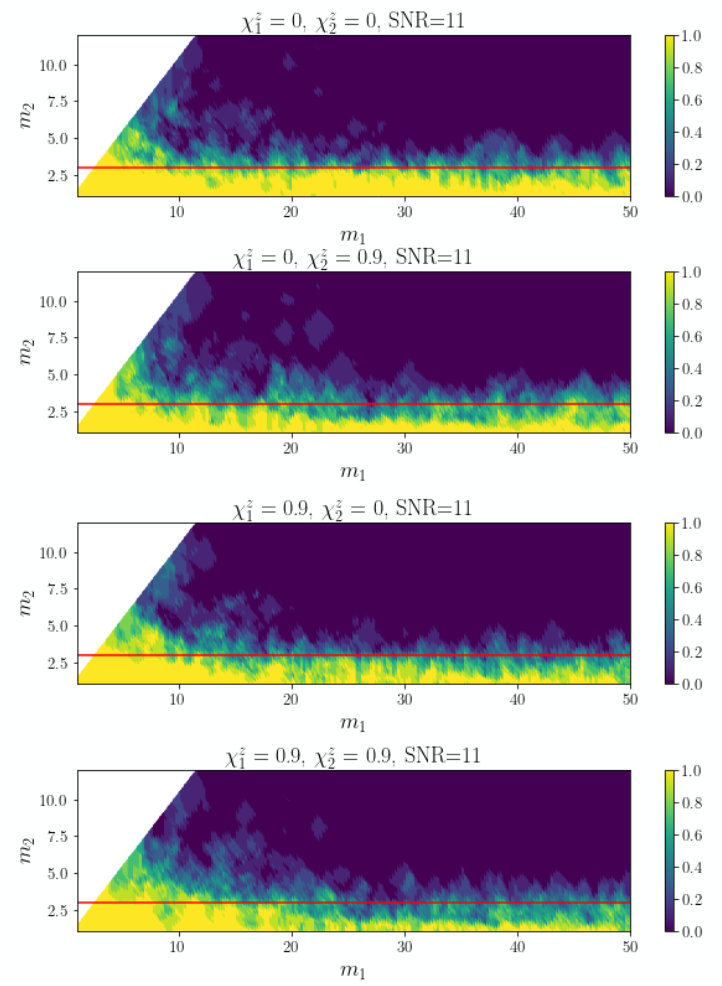
\includegraphics[width = 0.4\textwidth]{plot_fig4_chatt_spins.png}
  %   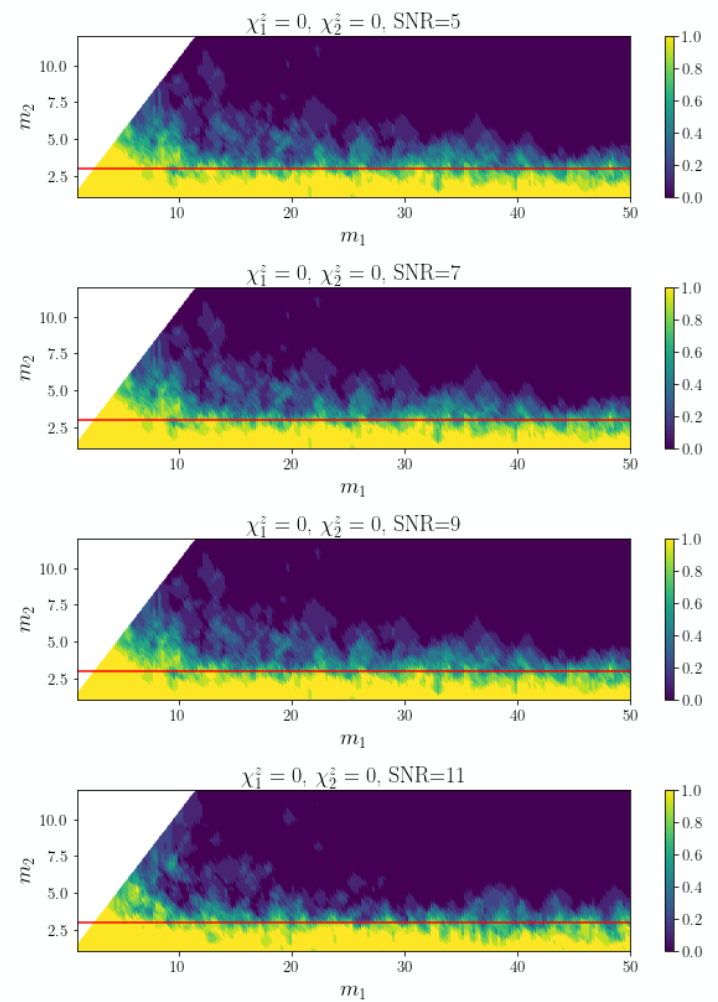
\includegraphics[width = 0.4\textwidth]{/Users/miquelmiravet/Projects/IPAM_LA/ML_group/IPAM2021_ML/algo/classy_KNN/PLOTS_KNN/NS_set/plots_miq/plot_fig4_chatt_snr.png}
   % \caption{Probability of having a neutron star in the binary system as a function of the values of the masses. The different panels show the results for different spins. The solid red line depicts the threshold mass for $m_2$.}
  %  \label{fig:m1m2}
%\end{figure}

%\begin{figure}
%	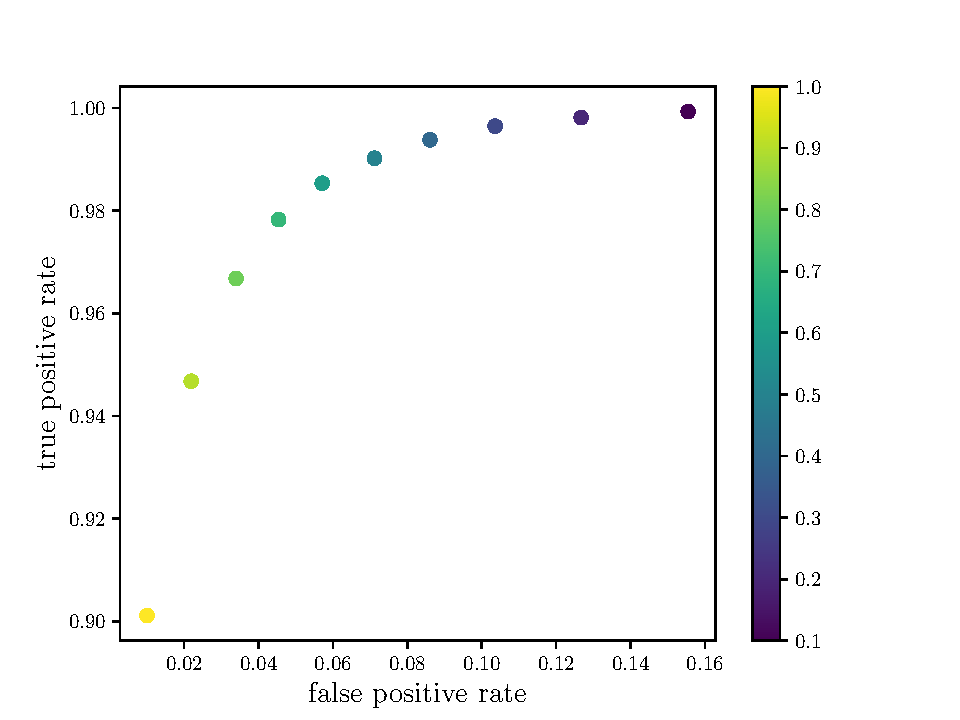
\includegraphics[width =0.4\textwidth]{ROCplot_NS.pdf}
  %  \caption{Relation of the true and false positive rates as a function of the threshold applied to make the decision between having or not having a neutron star. }
 %   \label{fig:roc}
%\end{figure}

%\mmt{The confusion matrix appears in Fig.~\ref{fig:confmat}. It depicts that the number of events that are correctly classified when there is a NS is much higher than the ones without a NS. The probability as a function of $m_1$ and $m_2$  is shown in Figs.~\ref{fig:m1m2}, There are no big differences with different values of the spins, but the most remarkable one is that the model classifies better for 0-spin values, especially when $m_1$ is large. The true and false positive rates in terms of the threshold probability (ROC curve) appear in Fig.~\ref{fig:roc}.}

%\subsubsection{\mmt{Has REM}}
%\mmt{In order to classify the events between having or not a post-merger remnant and therefore a likely EM emission, we apply again the cross validation to get the optimal number of neighbors, which turns out to be $K_{\rm REM} = 6$. Fig.~\ref{fig:crossvalK_REM} shows the dependence of the mean score with $K$ for this label. In this case, it is clearer that the score peaks at a certain value of $K$. Another hyperparameter that we change is the way the neighbors are weighted; in this case, we weight them with the inverse of the distance. } 

%\begin{figure}
 %   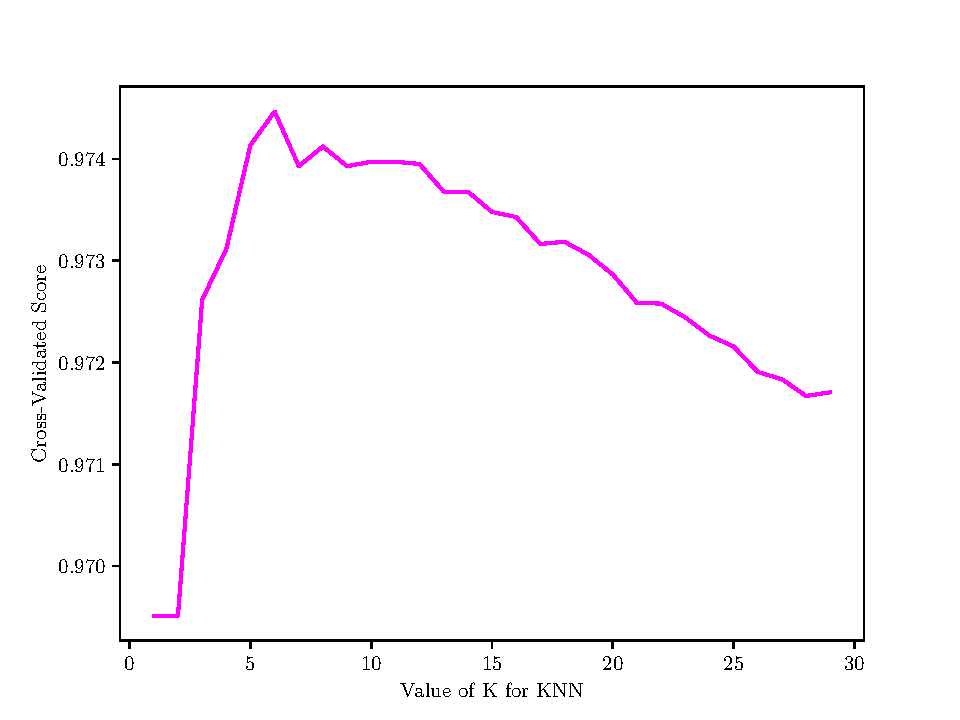
\includegraphics[width = 0.4\textwidth]{CrossValK_REM.pdf}
  %  \caption{Score of our KNN model as a function of the number of neighbors. We are considering \textit{HasREM}.}
  %  \label{fig:crossvalK_REM}
%\end{figure}

%\begin{figure}
 %   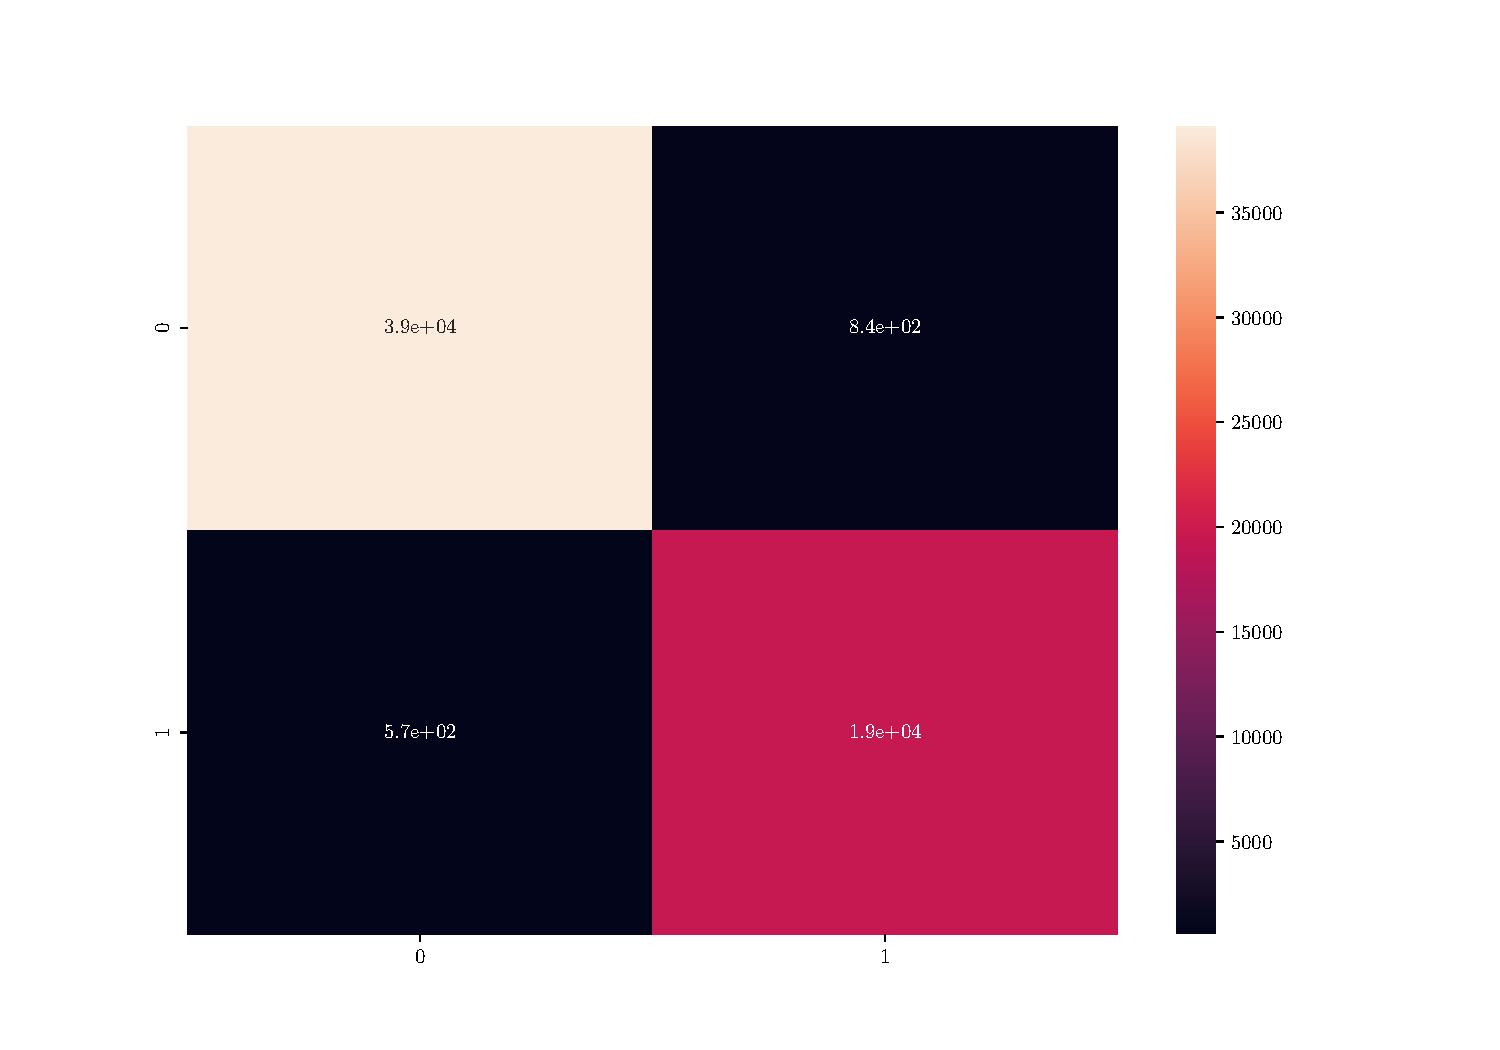
\includegraphics[width=0.45\textwidth]{conf_matrix_REM.pdf}
  %  \caption{Confusion matrix for our model for \textit{HasREM}, using the independent recovered values. }
  %  \label{fig:confmat_REM}
%\end{figure}

%\mmt{The confusion matrix depicted in Fig.~\ref{fig:confmat_REM} shows that the algorithm classifies correctly those events that do not have any remnant after the merger. On the other hand, it has more problems when classifying events with a post-merger remnant, i.e., with at least a neutron star with a mass $M_{\rm NS} \lesssim 2.83$ $M_{\odot}$ [MMT: Maybe this should go somewhere else]. There is also a dependence on the value of the spin that can be seen in Fig.~\ref{fig:m1m2_REM} [MMT:it would be nice to use the plots with the red line that Marina got].This dependence is correct, since the probability of having a remnant increases for large values of $m_1$ at larger spin, but this dependence is given by the EOS.  We show in Fig.~\ref{fig:roc_REM} the ROC curve for this new case.}

%\begin{figure}
 %   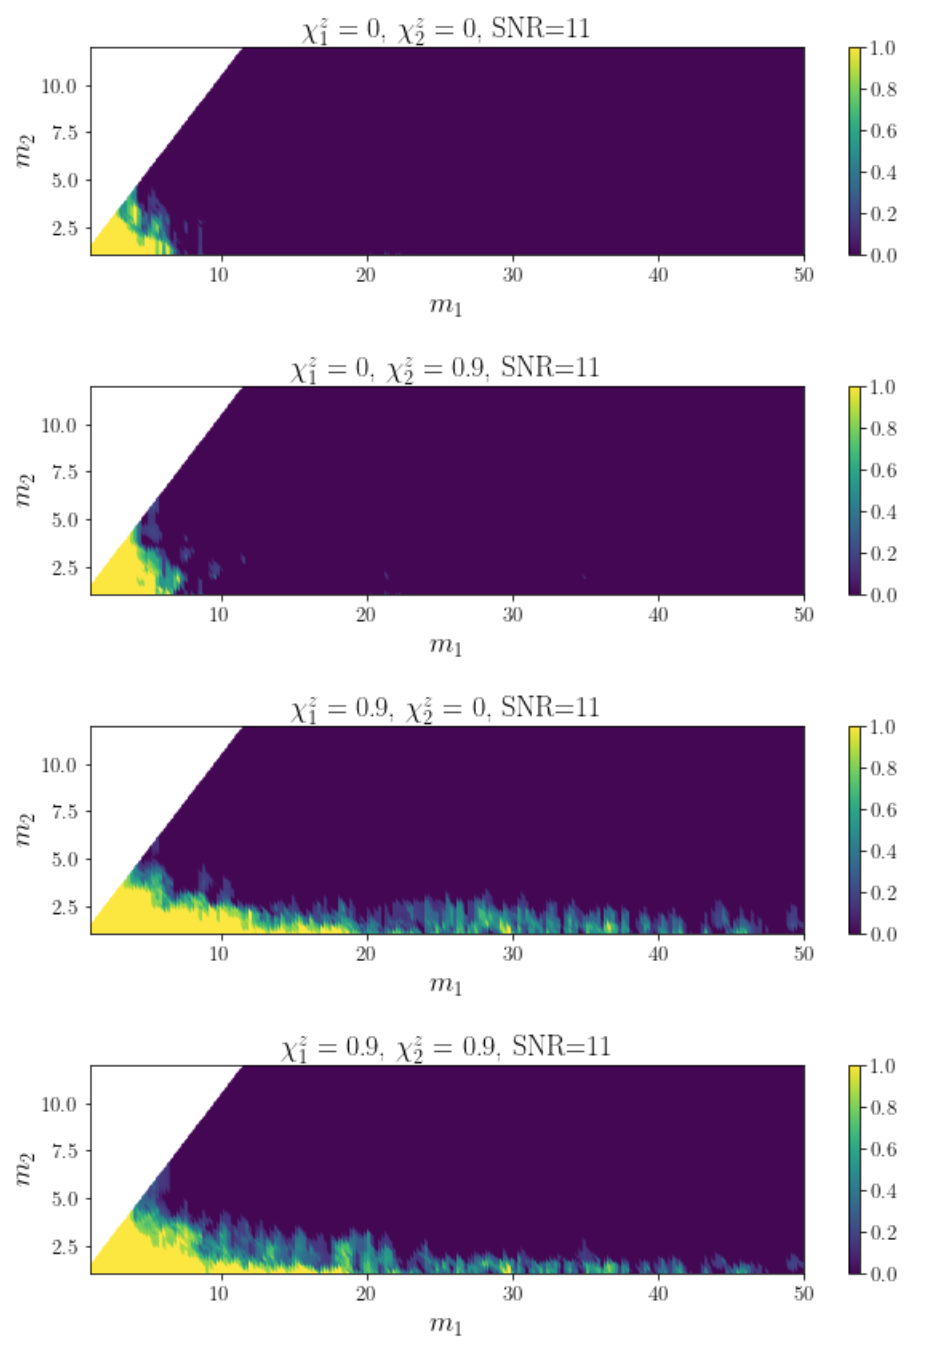
\includegraphics[width = 0.4\textwidth]{plot_fig4_chatt_spins_REM.png}
 %   \caption{Probability of having a remnant as a function of the values of the masses. The different panels show the results for different spins. }
%    \label{fig:m1m2_REM}
%\end{figure}

%\begin{figure}
%	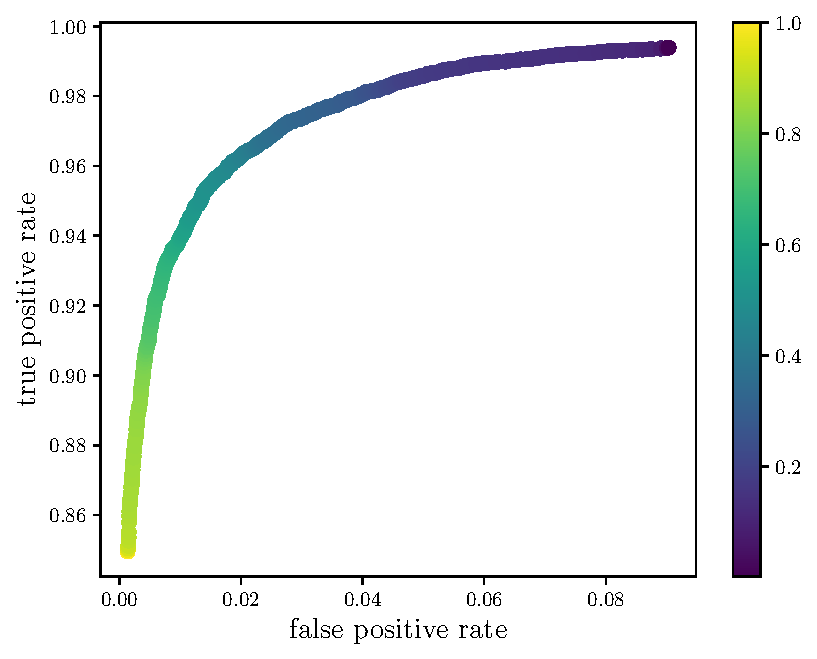
\includegraphics[width =0.4\textwidth]{ROCplot_REM.pdf}
 %   \caption{As in Fig.~\ref{fig:roc}, we show the relation of the true and false positive rates, but in this case as a function of the threshold applied to make the decision between having or not having a remnant object. }
 %   \label{fig:roc_REM}
%\end{figure}

%\mmt{[MMT: Nothing more to show here. These are the results I got for our KNN. It would be nice to plot the ROC curves for KNN and RF all together, and also the confussion matrices. I would like also to put a table comparing the different values of precision, sensitivity and score for both algorithms. More tests are needed with new datasets for KNN if we want an updated comparison.]}

